\section{Problem Description}
\label{sec:problem_description}
For a lab report you should dedicate this section to introducing necessary theory that you will later use to develop results and calculate necessary values, and present the experimental setup. It is probably a better idea in this case to structure your report in a section Background Theory and another section Experimental, where you should present how you have proceeded to produce your results in the latter of those two. For a report that is more theoretical, you could rather use the section Problem Description where you describe the experimental setup and the model equations you have developed for the particular system. This could for instance be a simplified steady state system for mass flows, as in Equation \eqref{eq:mass_balance}.
% Mass balance for a stationary system
\begin{equation}
    \label{eq:mass_balance}
    \hat{m}_{in} = \hat{m}_{out}
\end{equation}
Remember to explain all symbols that have been presented in the equations in text. In Equation \eqref{eq:mass_balance} $\hat{m}_{in}$ is mass flow into the system and $\hat{m}_{out}$ is mass flow out of the system. All symbols should appear in the text exactly as they do in the equations, hence the math shift is used to present the mass flows.
An example of an equation with fractions
\begin{equation}
    \frac
    {3\alpha + 2\alpha^2}
    {7\omega^3}
\end{equation}
An example of subequations
\begin{subequations}
    \label{eq:equation_set1}
    \begin{equation}
        \label{eq:equation_set1_a}
        \hat{m}_{1} = \hat{m}_{2} + \hat{m}_{3}
    \end{equation}
    \begin{equation}
        \label{eq:equation_set1_b}
        \hat{m}_{3} = \hat{m}_{2} + \hat{m}_{4}
    \end{equation}
\end{subequations}
You can reference the Equation set \eqref{eq:equation_set1} and its corresponding Subequation \eqref{eq:equation_set1_a} and \eqref{eq:equation_set1_b}.
All mathematical operators like sine and derivative should not be in italic, they are built in commands in \LaTeX and should be used as in Equation \eqref{eq:sine} and Equation \eqref{eq:derivative}. 
\begin{equation}
    \label{eq:sine}
    \tan (\theta) = \frac{\sin (\theta)}
                        {\cos (\theta)}
\end{equation}
\begin{equation}
    \label{eq:derivative}
    \diff{f}{x} = \lim_{h\to0}
                    \frac{f(x+h)-f(x)}
                        {h}
\end{equation}


It is good practice to include a picture of the setup as in Figure \ref{fig:setup}.
\begin{figure}[htb]
    \centering
    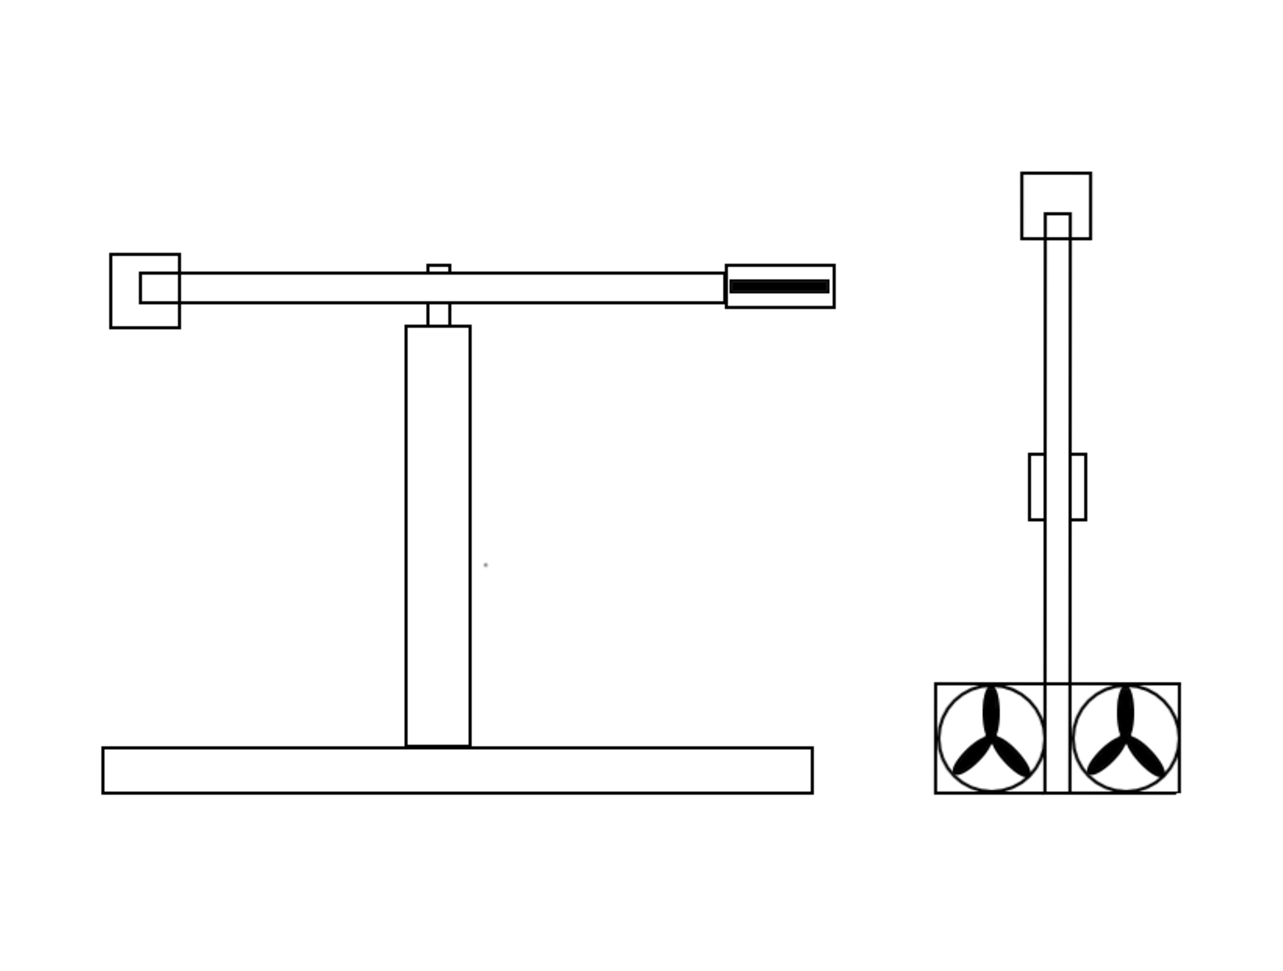
\includegraphics[scale=0.5]{Problem_description/figures/helikopter.eps}
    \caption{The figure shows the setup of the experiment performed.}
    \label{fig:setup}
\end{figure}
